\documentclass[12pt,letterpaper,addpoints]{exam}
\usepackage[utf8]{inputenc}
\usepackage{amsmath}
\usepackage{amsfonts}
\usepackage{amssymb}
\usepackage{amsthm}
\usepackage{graphicx}
\usepackage{tabularx}
\usepackage[left=2cm,right=2cm,top=2cm,bottom=2cm]{geometry}
\usepackage{multicol}
\usepackage{multirow,array}
\usepackage{newtxtext,newtxmath}
\usepackage{lastpage}
\usepackage{enumitem}
\newcolumntype{Y}{>{\centering\arraybackslash}X}
\firstpageheader{}{}{\includegraphics[scale=0.5]{BHCClogoBW.jpg}\hspace{-40pt}\vspace{-50pt}}
\firstpagefooter{}{}{Page \thepage ~of \pageref{LastPage}}
\runningheader{ \textsc{Math 181 First Exam Practice D}}{}{ \textsc{Fall 2018}}%{\includegraphics[scale=.5]{BHCClogoBW.jpg}\vspace{-10pt}}%\hspace{-60pt}\vspace{-10pt}}
\runningheadrule
\runningfooter{}{}{Page \thepage ~of \pageref{LastPage}}
\renewcommand{\thequestion}{{\bf Q\arabic{question}}}
%\renewcommand{\questionlabel}{{\thequestion .}}
%\pointformat{\fbox{\themarginpoints \,pt}}
%\pointsinrightmargin
%\setlength{\rightpointsmargin}{1.5cm}
%\pointsinmargin
%\setlength{\marginpointssep}{10pt}

\begin{document}

\newcommand{\AND}{~\textsc{and}~}
\newcommand{\OR}{~\textsc{or}~}

\begin{center}
\text{ }\\
\vspace{40pt}
\textsc{{\Huge Math 181 First Exam Practice D}}\\\vspace{5pt}
\textsc{{\large Spring 2019}}\\
\vspace{60pt}
\makebox[\textwidth]{\large Name:\enspace\hrulefill}\\
\vspace{40pt}
\fbox{\fbox{\begin{minipage}{6in}
\vspace{0.2in}
\begin{itemize}
\item Write your {\bf full name} on the line above.
\item Show your work. Incorrect answers with work can receive partial credit.
\item Attempt every question; showing you understand the question earns some credit.
\item If you run out of room for an answer, continue on the back of the page. Before doing so, write ``see back'' with a circle around it.
\item You can use 1 page (front and back) of notes.
\item You can use (and probably need) a calculator.
\item You can use the Geogebra Scientific Calculator instead of a calculator. You need to put your phone on {\bf airplane mode} and then within the application, start {\bf exam mode}; you should see a green bar with a timer counting up.
\item If a question is confusing or ambiguous, please ask for clarification; however, you will not be told how to  answer the question.
\item {\bf Box your final answer}.
\item A formula sheet is attached to this test.
\vspace{0.2in}
\end{itemize}
\end{minipage}
\begin{minipage}{0.2in}\text{ }\end{minipage}}}
\vfill
Do not write in this grade table.\\
\gradetable[h][questions]\\
\vfill
\end{center}

%%%%%%%%%%%%%%%%%%%%%%%%%%%%%%%%%%%%%%%%%%%%%%%%%%%%%%%%%%%%%%%%%%%%%%%%%%%%%%%

\newpage

\rhead{\textsc{Definitions and Formulas}}
{\bf Sample statistics:}\vspace{-10pt}
\begin{multicols}{2}\noindent
$n=\text{sample size} $\\
$x_i=\text{the $i$th value in a sample} $\\
$\bar x = \text{sample mean}$\\
$s = \text{sample standard deviation}$\\\\
$\bar x = \cfrac{\sum_{i=1}^n x_i}{n}$

\columnbreak \noindent
$Q_1$ = first quartile\\
$m$ = median\\
$Q_3$ = third quartile\\
IQR = inter-quartile range = $Q3-Q1$\\\\
$s = \sqrt{\cfrac{\sum_{i=1}^n (x_i-\bar x)^2}{n-1}}$ 
\end{multicols}

{\bf Population parameters:}\\
$\mu = \text{population mean}$\\
$\sigma = \text{population standard deviation}$\\

{\bf Probability:}\\
$\Omega = \text{set of all possible equally likely outcomes}$\\
$A = \text{event A, a set of outcomes}$\\
$A^c = \text{The complement of }A$\\
$B = \text{event B, another set of outcomes}$\\
$|A| = \text{size of set, number of outcomes in } A$\\
$P(A) = \text{probability of }A$\\
$P(A \AND B) = \text{probability of both $A$ and $B$}$\\
$P(A \OR B) = \text{probability of either $A$ or $B$ (or both)}$\\
$P(A | B) = \text{probability of $A$ given $B$}$\\\\
$P(A) = \cfrac{|A|}{|\Omega|}$\\\\
$0 \le P(A) \le 1$\\
$P(A \AND B) = P(A) \cdot P(B|A)$\\
$P(A \OR B) = P(A) + P(B) - P(A\AND B)$\\
$P(A^c) = 1 - P(A)$
\\\\
$A$, $B$ are disjoint (mutually exclusive) ~~$\iff~~P(A\AND B) = 0$\\
$A$, $B$ are non-disjoint ~~$\iff~~P(A\AND B) > 0$\\
$A$, $B$ are exhaustive ~~$\iff~~P(A\OR B) = 1$\\
$A$, $B$ are complements ~~$\iff$~~ $A$, $B$ are disjoint and exhaustive ~~$\iff$~~ $B=A^c$\\
$A$, $B$ are independent ~~$\iff~~P(A\AND B) = P(A)\times P(B) ~~\iff~~ P(A|B)=P(A)$\\

{\bf Random variables and distributions:}\\
$X=$ random variable \\
$x_i=$ the $i$th possible value of $X$. (Notice different meaning here {vs.} sample statistics.)\\
$k=$ number of possible values of $X$.\\
$E(X)=\mu=$ expected value of $X$\\
$\sigma=$ standard deviation of $X$\\
$\mu = \sum_{i=1}^k  x_i \cdot P(X=x_i) $\\
$\sigma = \sqrt{\sum_{i=1}^k (x_i-\mu)^2 \cdot P(X=x_i)}$


\newpage
\lhead{\textsc{Math 181}}
\rhead{\textsc{First Exam Practice D}}
\begin{questions}
\question[10] For simplicity, pretend a lie detector {\bf beeps} when it detects a lie. Assume 30\% of people lie on a test. If someone lies, the detector beeps about 80\% of the time. If someone tells the truth, the detector stays silent about 70\% of the time.

If a detector beeps, what is the chance the person is lying?
\begin{parts}
\part Make a tree diagram.
\vfill
\vfill
\part Make a contingency table.
\vfill
\vfill
\part $P(\text{lying} | \text{beep}) =$ ~? 
\vfill
\end{parts}

\newpage

\question[10] In Boston, a study was performed to investigate the effectiveness of charter schools in raising MCAS (math test) scores. There were 18,000 students who entered a lottery to go to a charter school. About 9000 ``won'' the lottery, so they went to charter schools. The other 9000 continued in public schools. After 2 years, these students then took the MCAS test, which each student either passed or failed.
\begin{center}
\begin{tabular}{|c|c c|} \hline
        & pass & fail \\ \hline
charter & 5850 & 3150 \\
public  & 3600 & 5400 \\ \hline
\end{tabular}
\end{center}
\begin{parts}
\item Is this study observational or experimental?
\vfill
\item Can causal relationships be established?
\vfill
\item Describe the null hypothesis.
\vfill
\item Describe the alternative hypothesis.
\vfill
\item Which treatment (charter or public) had a higher proportion of students pass the test?
\vfill
\item Do you think this difference in proportion happened just due to chance? Why?
\vfill
\end{parts}

\newpage

\question[10] The wildlife museum suggests that in the US, your chance of dying in a car accident is 1 in 84. That seems a bit high, so let's check with a back-of-the-envelope calculation.

In the United States, about 33,000 people are killed by cars each year from a population of about 330,000,000. If we assume these deaths are randomly distributed, that means each year a US resident has a 0.01\% chance of dying by car. Let's assume this chance remains constant and each year is independent.
\begin{parts}
\part What is the probability of a US resident not dying by car this year?
\vfill
\part What is the probability of a US resident not dying by car for 100 years?
\vfill
\part What is the probability that a US resident will die by car at least once over the next 100 years? 
\vfill
\end{parts}

\newpage

\question[10] Seven randomly sampled drivers in Massachusetts calculated their yearly cost of owning and operating an automobile (in thousand USD). (The US average is about \$9000 per year.)
\begin{center}
\begin{tabular}{c c c c c c c}
5.7 & 13.1 & 9.8 & 7.1 &  15.5 & 6.3 & 4.1
\end{tabular}
\end{center}
\begin{parts}
\part Calculate the sample mean. 
\vfill
\part Calculate the sample standard deviation. 
\vfill
\part Construct a boxplot of these data.
\vfill
\vfill
\end{parts}

\newpage

\question[10] Consider the three events depicted in the Venn diagram below.
\begin{center}
\includegraphics[scale=0.6]{figures/venn.pdf}
\end{center}
\begin{parts}
\part Evaluate $P(A)$.
\vfill
\part Evaluate $P(B)$.
\vfill
\part Evaluate $P(C^c)$.
\vfill
\part Evaluate $P(A|B)$.
\vfill
\part Evaluate $P(B^c|C)$.
\vfill
\part Evaluate $P(A \AND B)$.
\vfill
\part Evaluate $P(A \OR C)$.
\vfill
\part Which two events are independent? How do you know?
\vfill
\part Which two events are disjoint (mutually exclusive)? How do you know?
\vfill
\part Are these three events exhaustive? How do you know?
\vfill
\end{parts}

\newpage

\question[10] Pip rolls a 4-sided die (marked 1, 2, 3, 4) and flips a coin (marked 1, 2). Pip takes the sum. This process results in the probability distribution below, where the random variable $Y$ represents the sum.
\\{\Large
\begin{tabular}{|c|c|}\hline
$y_i$ & $P(Y = y_i)$\\\hline
2 & 0.125 \\
3 & 0.25 \\
4 & 0.25 \\
5 & 0.25 \\
6 & 0.125 \\ \hline 
\end{tabular}
}

\begin{parts}
\part Evaluate $P(Y=5)$.
\vfill
\part Evaluate $P(Y=1)$.
\vfill
\part Evaluate $P(2\le Y \le 4)$.
\vfill
\part Find the expected value (mean) of this probability distribution.
\vfill
\part Find the standard deviation of this probability distribution.
\vfill
\end{parts}


\end{questions}
\end{document}
